% siminos/atlas/cut.tex  pdflatex atlas
% $Author$ $Date$

\section{Poincar\'e sections}
\label{s:cut}

In general there are two strategies for replacing a continuous-time flow
by iterated mappings; by cutting it by Poincar\'e sections, or by
\emph{strobing} it at a sequence of instants in time. While
`strobing' is what any numerical integrator does, by representing a
trajectory by a sequence of time-integration step separated points,
strobing is in general not a reduction of a flow, as the sequence of
strobed points still resides in the full \statesp\ $\pS$, of
dimensionality $d$.

In the {\em Poincar\'e section method} one records the coordinates of a
trajectory whenever the trajectory reaches a
triggering event. A Poincar\'e section (or, from now on,
just a `section') is {\em not} a projection onto a lower-dimensional space:
Rather, it is a local change of coordinates to a direction along the
flow, and the remaining coordinates (spanning the section) transverse to
it. No information about the flow is lost; the full
space trajectory can always be reconstructed by integration from the
nearest point in the section.

    \ifdraft\color{blue}
        There is always tension between mathematics - linear problem eigenmodes
        (Fourier for translations and rotations) and physics - the fact that
        nonlinear dynamics states are far away from such axes, as they
        always involve a number of such linear modes strongly entangled.
    \color{black}\fi




\subsection{R\"ossler {\poincBord}}

As an example let of take the classic system of R\"ossler\rf{ross}

\index{R\"ossler system}
\beq
\begin{split}
  \dot{x} &= -x \,-\,z \\
  \dot{y} &= x + a y \\
  \dot{z} &= b + z (x - c)
  \label{eq:Rossler}
\end{split}
\eeq
where $a = b = 0.2$ and $c = 5.7$.
    \PC{
    Draw (un)stable eigenvectors as in \reffig{fig:AmLeAg06Im1}. Also, run
    the unstable spiral(s) for the upper brunch further out, to trace out the
    basin boundary.}

%%%%%%%%%%%%%%%%%%%%%%%%%%%%%%%%%%%%%%%%%%%%%%%%%%%%%%%%%%%%%%%%%%%%%
\begin{figure}
  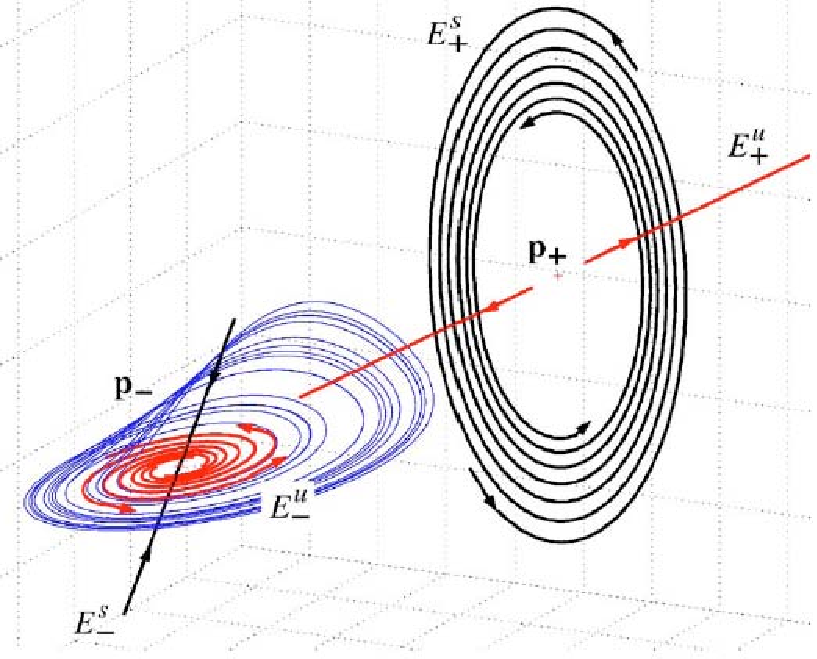
\includegraphics[width=0.3\textwidth]{AmLeAg06Im1}
    \caption{[From \refref{AmLeAg06}]
R\"ossler \eqva\ and their invariant manifolds. The stable manifold of
the inner {\eqv} $\ssp_{-}$  is 1-dimensional and the unstable one is a
spiral-out focus. The stable manifold at the outer {\eqv} $\ssp_{+}$ is a
spiral-in focus and the unstable manifold is 1-dimensional.
    }
\label{fig:AmLeAg06Im1}
\end{figure}
%%%%%%%%%%%%%%%%%%%%%%%%%%%%%%%%%%%%%%%%%%%%%%%%%%%%%%%%%%%%%%%%%%%%%

\subsection{R\"ossler two-chart atlas}
\subsection{R\"ossler unstable manifold curvilinear distance}
\subsection{R\"ossler return map}
\subsection{$N$-chart atlas, forward maps}
% \subsection{Ring of Fire return map\rf{lanCvit07}}

\section{Dynamics and symmetries: a recap}
\label{s:cutting}

\subsection{Group orbit}


    \ifdraft\color{blue}
%%%%%%%%%%%%%%%%%%%%%%%%%%%%%%%%%%%%%%%%%%%%%%%%%%%%%%%%%%%%%%%%%%%%%
\begin{figure}
   \centering
(a)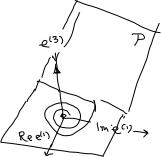
\includegraphics[width=0.20\textwidth]{A29PoincBad}
(b)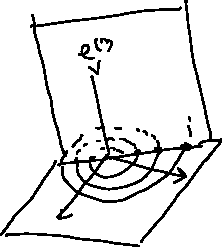
\includegraphics[width=0.20\textwidth]{A29PoincGood}
   \caption{\label{fig:A29PoincBad}
A Poincar\'e section should capture important features of the local flow.
    (a)
A section through a \template\ off the invariant set is bad, as it misses
dynamics around a nearby \eqv.
    (b)
If an \eqv\ is chosen as a \template, the section is good - it captures
all local dynamics.
}
\end{figure}
%%%%%%%%%%%%%%%%%%%%%%%%%%%%%%%%%%%%%%%%%%%%%%%%%%%%%%%%%%%%%%%%%%%%%

The two charts
\reffigs{fig:RoessSct1}{fig:RoessSct2} illustrate \poincBord,
and \reffigs{fig:RoessSctAtlas} the combined 2-chart atlas.

\begin{figure}%[H]
\begin{center}
  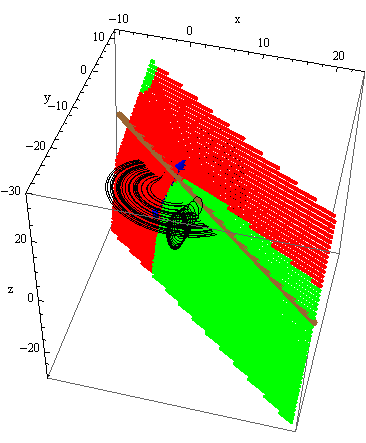
\includegraphics[width=0.30\textwidth,clip=true]{RoessSct1}
\end{center}\label{fig:RoessSct1}
  \caption{
  A Poincar\'e section for R\"ossler flow correctly centered on the inner
  {\eqv} $\ssp_{-}$ \template, as sketched in
  \reffig{fig:A29PoincBad}\,({\it b}).
}
\end{figure}

\begin{figure}%[H]
\begin{center}
  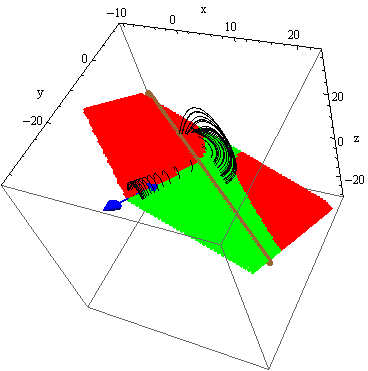
\includegraphics[width=0.30\textwidth,clip=true]{RoessSct2}
\end{center} \label{fig:RoessSct2}
  \caption[R\"ossler section, outer {\eqv}]{
  A Poincar\'e section for R\"ossler flow correctly centered on the outer
  {\eqv} $\ssp_{+}$ \template, as sketched in
  \reffig{fig:A29PoincBad}\,({\it b}).
  }
\end{figure}

\begin{figure}%[H]
\begin{center} \label{fig:RoessSctAtlas}
  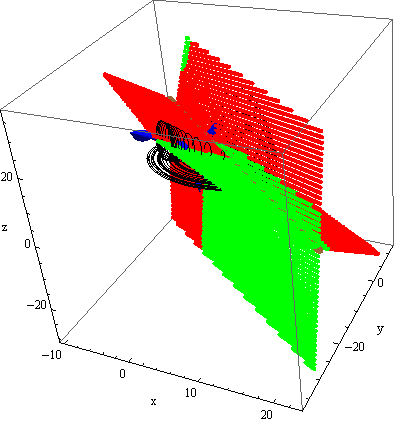
\includegraphics[width=0.30\textwidth,clip=true]{RoessSctAtlas}
\end{center}
  \caption{
  A two-section atlas for R\"ossler flow, with the local sections of
  \reffigs{fig:RoessSct1}{fig:RoessSct2} oriented and combined so the
  Euclidean distance from the first \template\ to the ridge (intersection
  of the two sections, indicated by the brown line in individual sections
  of the preceding figures), and then to the second \template\ is
  approximately minimized.
  }
\end{figure}

\begin{figure}
\begin{center}
(a) % 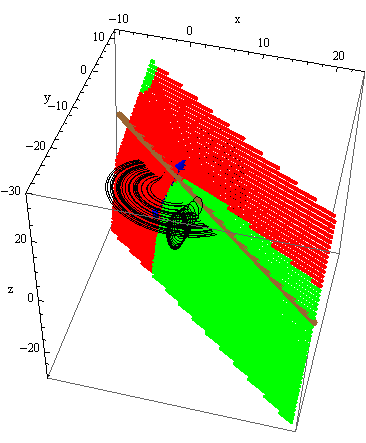
\includegraphics[width=0.30\textwidth,clip=true]{RoessSct1}
(b) 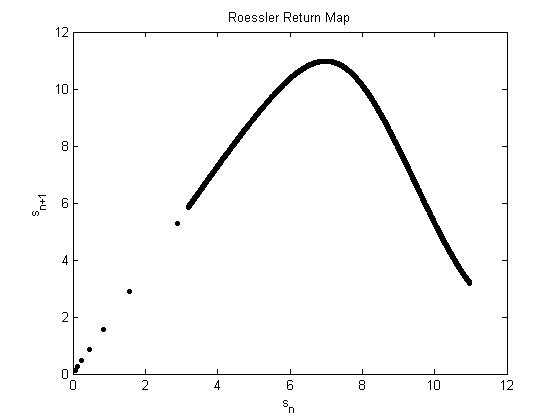
\includegraphics[width=0.30\textwidth,clip=true]{RoessRetMap}
\end{center}
  \caption{
(a) R\"ossler strange attractor section of \reffig{RoessSct1}
(b) R\"ossler return map for curvilinear distance as measured
along the unstable manifold section (the method of
\refref{Christiansen97}, see \refrefs{DasBuchBasu07}).
  }
\label{fig:RoessRetMap}
\end{figure}


Nature, she don't care :
turbulence breaks all symmetries

{\Large Das Problem}
Drifting is energetically cheap.
Flows are lazy, rather than do work, solutions drift along non-shape-changing
symmetry directions.

An example of a wurst is the set of group orbits traced out by a single
short \rpo\ in \reffig{fig:CLf01group}. As \cLe\ exhibits only the simplest,
$m=1$ Fourier mode, all group orbits are circles, which appear elliptical in
most $d=5 \to 3$~dimensions projections.
    \PC{define \cLe, refer to \reffig{fig:CLf01group}}
    \color{black}\fi

The \emph{group orbit} $\pS_\ssp $ of a \statesp\ point $\ssp \in \pS$ is
traced out by the set of all group actions
\beq
\pS_\ssp = \{\LieEl\,\ssp \mid \LieEl \in {\Group}\}
% \,,\qquad \pS_\ssp \subset \pS
\,.
\ee{sspOrbit}
Any state in the  group orbit set $\pS_{\ssp}$
is physically equivalent to any other. The action of a symmetry group
thus stratifies the \statesp\ into a union of group orbits,
\reffig{fig:BeThTraj}\,{(a)}.

\subsection{Norms - distances between states}

We have seen that in presence of the continuous $\SOn{2}$ symmetry
\reqva\ and \rpo s are 2- and 3-dimensional manifolds of physically
equivalent states. How are we to compare a pair of such states? We shall
do this here by determining the minimal distance between them.

In order to quantify
whether two fluid states are close to or far from each other, one
needs a notion of distance between two points in \statesp, measured
here as
\beq
  \Norm{\ssp-\ssp'}^2  = \braket{\ssp-\ssp'}{\ssp-\ssp'} =
\frac{1}{V}
\int_\bCell \! d \bx \;
(\vec{u}-\vec{u}') \cdot (\vec{u}-\vec{u}')
\,,
\ee{innerproduct}
invariant under all symmetries of the flow,
$\Norm{\ssp-\LieEl\,\slicep}=\Norm{\sspRed-\slicep}$
There is no compelling reason to use this {`energy norm'}, other than
that velocity fields is what is generated in a numerical
computation. What norm one actually uses depends very much on the
application; the importance (and arbitrariness) of the choice of
norm cannot be overemphasized. For example, in the study of `optimal perturbations' that
move a laminar solution to a turbulent one, both energy
\citep{TeHaHe10} and dissipation \citep{LoCaCoPeGo11} norms have been
used.
For experimental data sets, pattern recognition type norms could be the
only practical option\rf{MakeThisUp}.

\subsection{\Statesp\ visualization}

On perils of thinking linearly: bases such as Fourier modes are
perfectly natural for problems such a bifurcation of a steady state, and
other weak perturbations. They are absolutely unnatural for strongly
nonlinear problems, with many Fourier modes of comparable magnitude and
strongly entangled.

\subsection{\CLe}
\subsection{Experimentalist description: a video 1D to 3D arrays of pixels}
\subsection{Theorist description: $\infty$-\dmn\ \statesp}
\subsection{Time orbit: point is a point, line is a line in all dimensions}
\label{sect:TimeOrb}

\subsection{Physical dimension: covariant Lyapunov vectors}
